\documentclass{article}

% if you need to pass options to natbib, use, e.g.:
%     \PassOptionsToPackage{numbers, compress}{natbib}
% before loading neurips_2020

% ready for submission
% \usepackage{neurips_2020}

% to compile a preprint version, e.g., for submission to arXiv, add add the
% [preprint] option:
%     \usepackage[preprint]{neurips_2020}

% to compile a camera-ready version, add the [final] option, e.g.:
%     \usepackage[final]{neurips_2020}

% to avoid loading the natbib package, add option nonatbib:
     \usepackage[nonatbib]{neurips_2020}

\usepackage[utf8]{inputenc} % allow utf-8 input
\usepackage[T1]{fontenc}    % use 8-bit T1 fonts
\usepackage{hyperref}       % hyperlinks
\usepackage{url}            % simple URL typesetting
\usepackage{booktabs}       % professional-quality tables
\usepackage{amsfonts}       % blackboard math symbols
\usepackage{nicefrac}       % compact symbols for 1/2, etc.
\usepackage{graphicx}
\usepackage{microtype}      % microtypography


\title{YOLO-Vacant Parking Spot Detector}

% The \author macro works with any number of authors. There are two commands
% used to separate the names and addresses of multiple authors: \And and \AND.
%
% Using \And between authors leaves it to LaTeX to determine where to break the
% lines. Using \AND forces a line break at that point. So, if LaTeX puts 3 of 4
% authors names on the first line, and the last on the second line, try using
% \AND instead of \And before the third author name.

\author{%
  Andrew Park \\
  Electrical and Computer Engineering\\
  A17406465\\
  % examples of more authors
  \And
  Minsang Kim \\
  Electrical and Computer Engineering\\
  A16636382 \\
}

\begin{document}

\maketitle

\begin{abstract}
    Not only within UCSD campus, there are numerous isseus related to finding
    parking spots nearby. Therefore, the technology to annoatate the available parkint
    spot at a specific parking lot is damanded. To implement the artificial intelligence
    model, CNN is implemented to annoatate the avaiblable parking spot. During
    implementation, we used the dataset for image-based parking space occupancy to collect data for parking structure
    to train the architecture. We will display the resulting image, the overall accuracy,
    and the loss of the model. 
    

\end{abstract}

\section{Introduction}

Finding a vacant parking space in a given lot is a tedious and costly task: a person must drive through the whole parking lot in order to find a vacant space. This uneffective process will 
waste gasoline and time while searching for a parking space. Furtermore, this will cause congestion in the parking lot. Therefore, by displaying the occupancy of spaces in a given parking lot
will significantly reduce the time cost, traffic congestion, and gasoline consumption. YOLO-Parking will aid this wasteful process by displaying vacant and
occupied parking spaces. Although there are existing methods to detect the occupancy of a parking space, such as car detector on every parking space and other object detector architectures 
that detects the occupancy, most of them are expensive or slow in detecting parking spots\cite{DBLP:journals/corr/abs-2107-12207}. Furthermore, there are several traditional models  models 
to detect the instance segmentation of a vacant parking spot, but they are slow in detection for videos. 

In this paper, we propose a new model to detect vacant parking spots: You Only Look Once (YOLO). YOLO architecture is one of the fastest architecture that accurately performs object detection \cite{redmon2016look}. 
Additionally, several cameras mounted in the parking lot to detect vacancy of a space is relatively cheaper than placing a car detector on every parking space in a parking lot \cite{DBLP:journals/corr/abs-2107-12207}. 



\section{Related Work}

\textbf{R-CNN} \quad R-CNN \cite{DBLP:journals/corr/abs-2107-12207} is a widely used object detecting CNN model with relatively high accuracy. The first step is to regional proposal using selective search methods to propose bounding box. 
Then, for each region proposal, the model warped the propsed regions to use them as inputs for a convolutional neural network. The CNN classifies eacn input proposed region using SVM specific to a class \cite{girshick2014rich}. 
However, the training rate is slow due to large number of parameters to learn, and the inference rate is also slow. In one of the previous approaches in detecting parking spots, Martin Marek proposed R-CNN: the model first pool 
proposed parking spot patches in the original image and then a CNN produces a binary output whether the space in each patch is occupied or not \cite{DBLP:journals/corr/abs-2107-12207}. The authors provided two methods for pooling
for the first step in R-CNN: the interpolation of pixels to construct quadrilateral bounding boxes and construction of minimal bounding boxes \cite{DBLP:journals/corr/abs-2107-12207}. 

\textbf{Faster R-CNN FPN} The input image first undergoes a feature pyramid network (FPN). Then, the authors extract the features of the parking spots and pass them through respective classification head for classification. However, 
the input image must be resized, thus limiting the output image from being full resolution \cite{DBLP:journals/corr/abs-2107-12207}. Both R-CNN and R-CNN is still slow in inference for object detection in videos. Faster R-CNN can use
one of the two methods of pooling mentioned above \cite{DBLP:journals/corr/abs-2107-12207}. 

These two models are merely the baseline of parking vacancy object detector using CNN. In this paper, we intend to improve the model in inference time by using YOLO model. 

\section{Method}

\subsection{Model}
We began the project with instance segmentation method to determine the pixels of the parking spots. However, it was extremely difficult to find the appropriate dataset for instance segmentation of parking lots. Furthermore, it was not necessary to classify
each pixel to detect vacant space. Rather, we merely wanted to count the number of vacant spaces available in the given parking structure and relative spot of vacancy in a given parking lot. This is the reason why we chose neural network models that are capable 
of object detection. 

We decided to use the popular model proposed by Joseph et al. \cite{redmon2016look} You Only Look Once because of its speed and accuracy. Compared to the speed of the YOLO architecture in object detecting, the model itself is surprisingly simple. Given an image, 
the model first resizes the image to a resolution of $448 \times 448$. The resized image is divided into $S \times S$ 
grid and is passed through convolutional neural network. The model consists of 24 convolutional layers with two fully connected layers following the convolutional neural network. During the process of convolutional network, the model simultaenously
draw bounding boxes and predicts the probability that each grid contains a class. The prediction of the model is an $S \times S \times (B * 5+C)$ tensor. In our case, we are evaluating whether the space is occupied or not, so the number of classes 
$C = 2$. The size of the grid for division $S = 7$ and the number of bounding boxes is  $B$. Each prediction for bounding box consists of 5 values: center $(x,y)$, height, width, the confidence value. Since there are $B=2$ bounding boxes, the prediction 
tensor contains $2 * B = 10$ values. The other $C=2$ values are the conditional probability that the given object is the i-th class: $P(C_i | Object)$. The confidence probability is calculated by the IOU of each bounding box \cite{redmon2016look}. 

\begin{figure*}[ht]
    \centering
    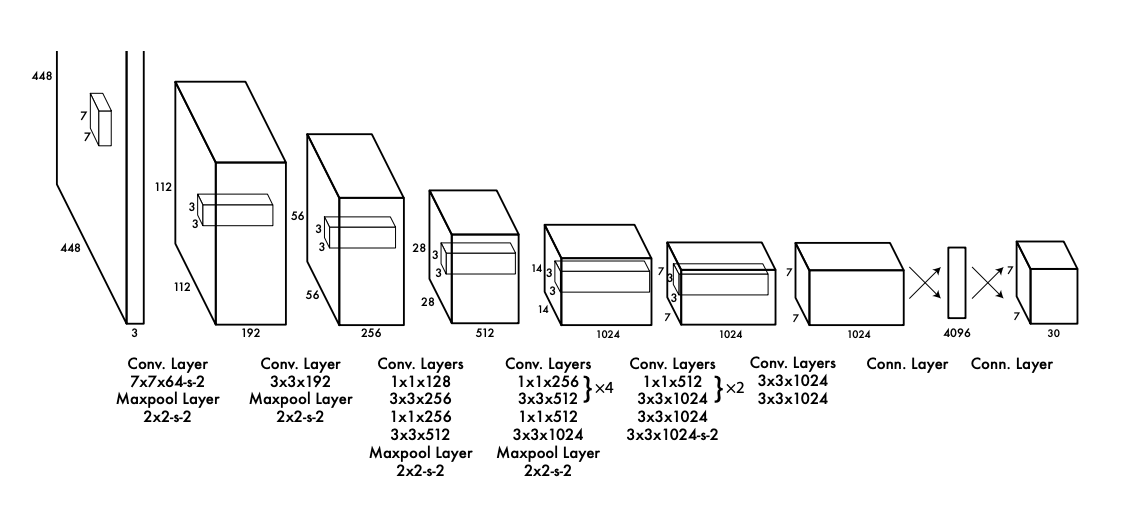
\includegraphics[width=0.9\textwidth]{figs/Screenshot 2024-03-22 at 21.55.19.png}
    \caption{YOLO Architecture}
\end{figure*}

To reduce the training time, we collected pretrained parameter in the backbone of the YOLO architecture. This is a unconventional architecture for vacant parking spot detection. This architecture is faster than other conventional model, such as R-CNN and Faster R-CNN \cite{redmon2016look}. 
Therefore, this model can be used in video cameras mounted in the parking lot to detect parking spaces in live footages. 


\begin{itemize}
    \item training algorithm, testing algorithm.
    \item what is the new proposed techniques compared to previous work, and the reason and strength of choosing the method.
\end{itemize}

\section{Experiments}

\subsection{Dataset}
For the dataset, Parking Space Image Dataset is used. The dataset consists of parking lot images and  

\subsection{Results}

The following figures are the results after training the model: 
\begin{figure*}[ht]
    \centering
    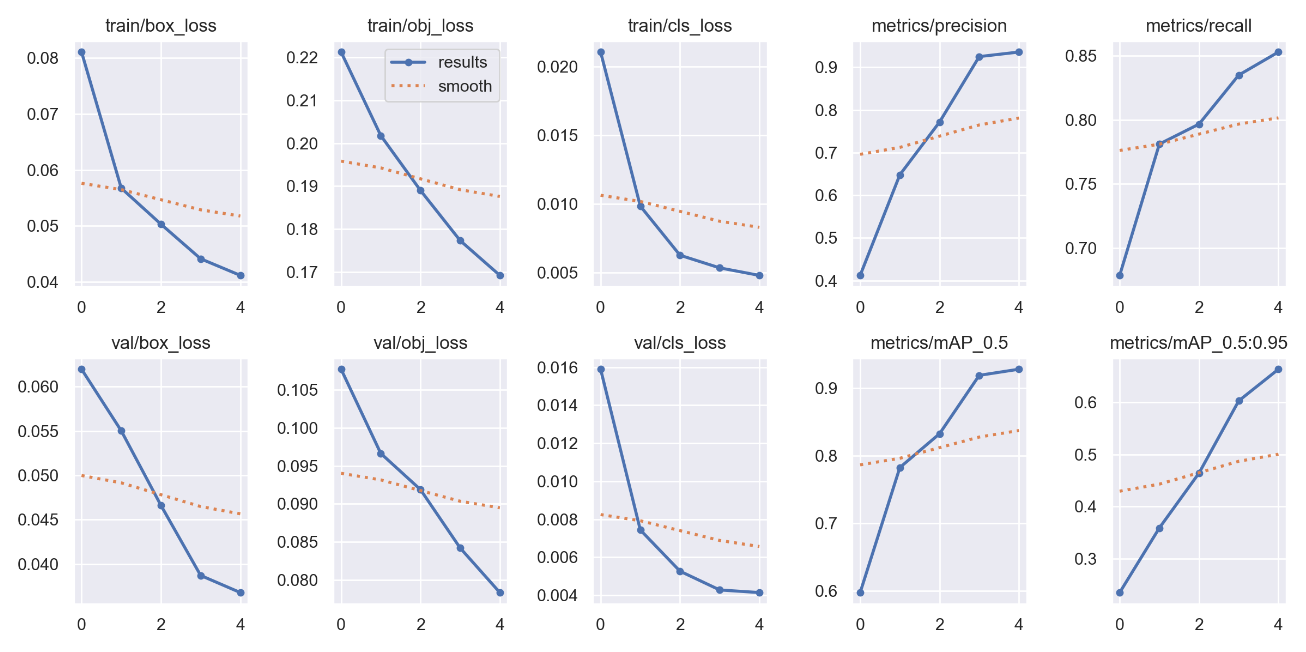
\includegraphics[width=0.9\textwidth]{figs/loss-function.png}
    \caption{Loss Function Over Epochs}
\end{figure*}
\begin{figure*}[ht]
    \centering
    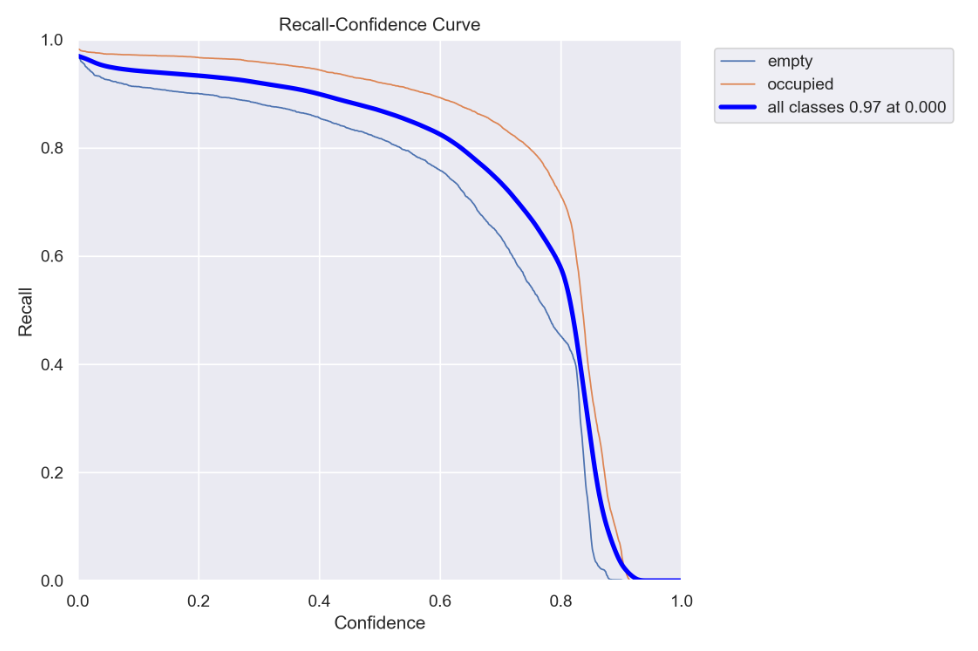
\includegraphics[width=0.45\textwidth]{figs/recall-confidence.png}
    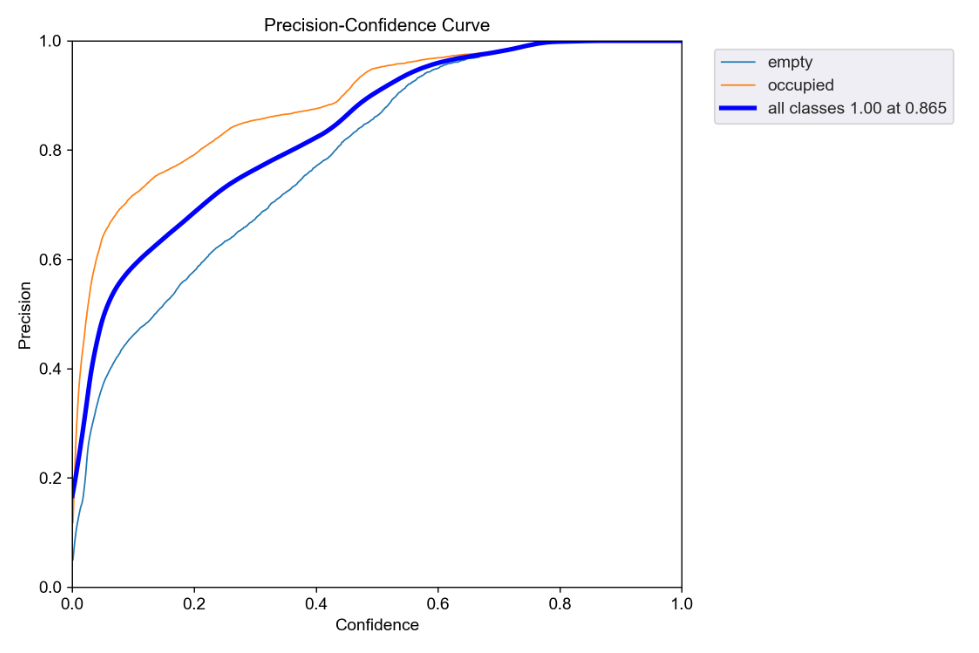
\includegraphics[width=0.45\textwidth]{figs/percision-confidence.png}
    \caption{Recall-Confidence Graph (left) and Confidence-Percision Graph (right) }
\end{figure*}

In this section, You should include the following things:

\begin{itemize}
    \item the datasets you use:
        \subitem the brief introduction of the dataset
        \subitem the data format
        \subitem other information related to your experiments
    \item your results
    \item ablation study on training your networks, how does the method work with more or less data, with/without some components (optional)
\end{itemize}


\section{Supplementary Material}

You should also include a video recording a presentation (with motivation, approach, results) for this project. 

\bibliographystyle{plain}
\bibliography{bibliography.bib}

\end{document}
